\section{Creating Rapport Agents using Rule-Based Approaches}
\label{sec:rulebasedAgents}

Rule-based systems are great for deterministic scenarios where the agent does not need to be as robust as other systems used in non-deterministic scenarios~\cite{Mutlu2006} where rules might not be easy to define. However, rule-based systems are not easily ported to other scenarios, nor are they as easily scalable because they are often based on more contextual conditions~\cite{Kok2012}.

\subsection{Gaze}
\label{sub:sec:gaze}

Gaze is an important aspect of rapport as it enhances the second component of rapport: mutual-attention. Following this, we present three different research work where researchers attempt to establish more harmonious relationships with users following different strategies.

Mutlu et al., implemented a scripted mutual gaze agent that synchronises gaze behaviour with pre-recorded voice and gestures~\cite{Mutlu2006}. In their experience, they concluded that participants would recall the story better when the robot looked at them more often. Additionally, using the same gaze frequency, women felt better when the storytelling agent gazed less at them. This is important if we want to develop agents for education scenarios where transmitting information is crucial.

Stanton et al., developed a robot assistant for a cooperative visual tracking game (the ``shell game'')~\cite{Stanton2014}. Volunteers would ask the robot for help. However, occasionally, the robot would volunteer to give an answer. In their experiment, they concluded that eye gaze can have powerful effects upon participant decision-making and behaviour, and influence their task performance. For example, humans tend to comply with the robot's suggestion when it gazed at them on harder tasks but, on easier tasks, gaze reduced trust. The authors postulate that ``robot gaze can have either a positive or negative impact upon trust and compliance, depending upon the nature of the robot’s request or suggestion''.

Andrist et al., developed a virtual agent focused on mutual gaze behaviour in a therapy scenario~\cite{Andrist2015} that would systematically swap its gazing target between the task area and the conversational partner's using tracking sensors. According to their study, matching gaze behaviour models to the user's personality increases motivation and engagement in repetitive tasks. In other words, different personalities require different rules (systemized in Table~\ref{table:gazetimes}). For example, between tasks, when therapists would provide encouragement, introverts shift more often their gaze to the therapist than extroverts.

\begin{table}[H]
	\centering
	\begin{tabular}{|l|l|l|l|l|}
	\hline
	\multicolumn{1}{|c|}{\textbf{Personality}} & \multicolumn{2}{c|}{\textbf{Extrovert}}  & \multicolumn{2}{c|}{\textbf{Introvert}}  \\ \hline
	\textbf{Phase}                             & \textbf{In-Task (s)} & \textbf{Between-task (s)} & \textbf{In-Task (s)} & \textbf{Between-task (s)} \\ \hline
	Partner                                    & 2.66 (0.80)      & 3.91 (1.22)           & 0.57 (0.19)      & 1.59 (0.39)           \\ \hline
	Puzzle                                     & 4.04 (2.12)      & 1.01 (1.26)           & 11.65 (11.17)    & 6.21 (8.14)           \\ \hline
	\end{tabular}
	
	\caption{Means and standard deviations of gaze duration to the partner, and to the puzzle. From~\cite{Andrist2015}}.
	\label{table:gazetimes}
\end{table}


\subsection{Behavioural Mimicry}

Behavioural mimicry is another important aspect of rapport as it enhances the third component of rapport: coordination.

It is well understood in Psychology that humans can convey empathetic responses via involuntary facial mimicry~\cite{Riek2009, Mancini2013, Chartrand1999}. Taking this into account, several researchers have been exploring how to use this information and improve current \ac{HRI} agents~\cite{Chartrand1999, Sidner2006, Hatfield1992}.

Laurel D. Riek et al., developed an autonomous robotic agent named Virgil capable of mimicking head gesture~\cite{Riek2009}. Similar to others experiments, the agent acted as a silent listener while participants answered open questions. In their experiment, albeit with low number they gathered some interesting remarks: it is possible to influence behaviour when subjects co-nod in return to Virgil's nod; subjects felt that they were interacting with an automated machine as it was unclear if the agent's head nods were a response to something the subject said or because he just did it; few participants perceived the agent's head movement as too ``erratic or jerky'' which might be more noticeable when the agent's head is static for notable periods; lastly, it was interesting that few participants suggested that the agent should make attentiveness signals such as ``Mm-hmmm'', which are formally backchannel, one of the main aspects of rapport.

\subsection{Emotional Contagion}
People are not insensible to their peers. In fact, there is evidence that our behaviour is able to change the emotional state of our conversational partner either deliberately (e.g., to persuade) or unintentionally triggering emotional responses~\cite{Dimberg2000, Chartrand1999, Hurley2012, Hess2010, Barsade2015}. As such, the research community as been investigating the impact of facial expressions on rapport in \ac{HRI} interactions~\cite{Melo2011, Wang2009}. Current evidence suggests that lower levels of disgust are correlated with lower levels of rapport however, the same evidence suggests that smile is not the best reliable mechanism to attest the quality of the interaction~\cite{Wang2009}.

Moreover, psychologists have remarked that people have the tendency to mimic facial expressions~\cite{Dimberg2000}. On their studies, they noticed that people trend to unconsciously mimic the same facial expression as the one they were exposed to.

\subsection{\acf{SERA}}
\label{sub:sec:SERA}

Tiago Ribeiro et. al. developed a framework that allows the integration of AI agents on a robotic body, in \ac{HRI} scenarios. The \acf{SERA} framework~\cite{Tullio2015} follows the SAIBA model~\cite{Kopp2006} and is very similar to \ac{ROS}~\cite{Quigley2009} due to, respectively, the separation between intention planning, behaviour planning and realisation, and due to the usage of decoupled modules in an asynchronous messaging system called \textit{Thalamus}. It aims to be used by both technical and non-technical developers such as psychologists~\cite{Tullio2015}, which is an advantage as their knowledge is crucial during the development and analysis of \ac{HRI}. For example, utterances are modelled using markup text that can contain non-interrupting behavioural actions that can be defined by non-technical teams collaboratively (Table~\ref{table:exampleutterances}).

\begin{table}[H]
	\centering
	\begin{tabular}{|l|l|l|}
	\hline
	\multicolumn{1}{|c|}{\textbf{Category}} & \multicolumn{1}{c|}{\textbf{Subcategory}} & \textbf{Utterance}  \\ \hline	
	intro & greet & \specialcell{Hi $|$\texttt{Name}$|$! $<$gaze(person)$>$} \\ \hline
	game & score & \specialcell{Yey!$<$Animate(surprise2)$>$}  \\ \hline
	game & results & \specialcell{Managed $<$Points$>$! $<$gaze(person)$>$} \\ \hline
	end & ending & \specialcell{I am glad to have met you! $<$animate(happy4)$>$} \\ \hline		
	\end{tabular}
	\caption{Set of utterances compatible with \acf{SERA}. Set of utterances compatible with \acf{SERA}. Actions are delimited by $<$ and $>$, and substitution variables by $|$.}
	\label{table:exampleutterances}
\end{table}

\subsubsection*{System description}

The most important elements of \ac{SERA} are:
\begin{itemize}
	\item \textbf{\textit{Thalamus}}: receives and delivers the published messages to the right subscribers;
	\item \textbf{\textit{Skene}}: translates high-level intentions into behaviour actions;
	\item \textbf{\textit{Nutty Tracks}}: animation engine;
	\item \textbf{\textit{Speech Server}}: \ac{TTS} engine. 
\end{itemize}

\textit{Skene} is the most relevant component in \ac{SERA} for the development of rapport agents as it is the controller that plans animations and non-verbal behaviours such as gaze, utterances and animations according to perceptual messages. This component is rule-based and has an explicit representation of its body position over his physical environment.

SERA also includes modules for bridging external tools such as FAtiMA to model emotions~\cite{Dias2011} or Unity to create virtual scenarios. All these modules co-exist inside the \textit{Thalamus} ``network'' to cooperate, in order to achieve the interactional goals in any \ac{HRI} scenario (e.g., negotiation scenarios on Figure~\ref{fig:SERA:Examples}).

\begin{figure}[H]
	\centering
	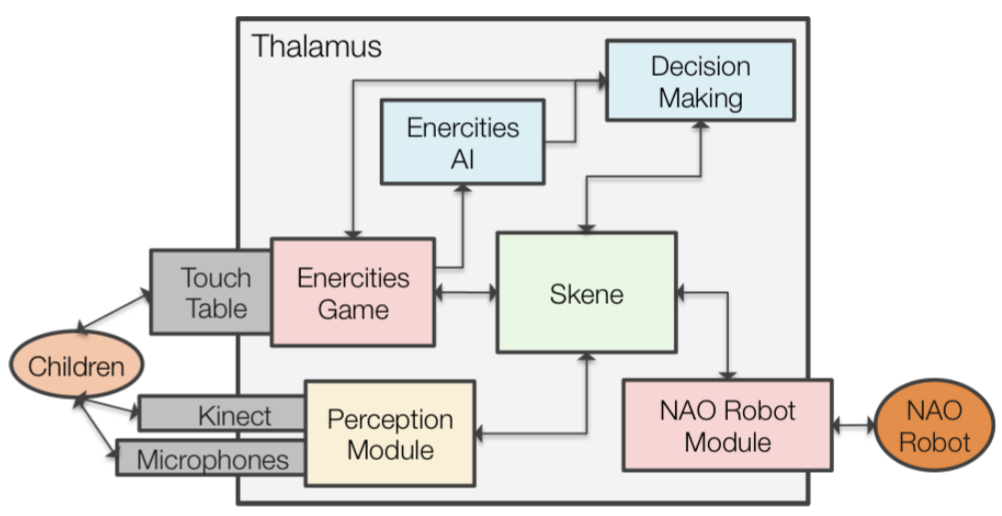
\includegraphics[width=0.6\linewidth]{images/SERA_ExSystemEC.png}
	\caption{Enercities scenario system architecture integrated with the SERA framework. From~\cite{Tullio2015}.}
	\label{fig:SERA:Examples}
\end{figure}

%Another example, using the Keepon robot~\cite{Kozima2009} (Figure~\ref{fig:robots:Keepon}) to keep ``early adolescents engaged in physical activity over long periods of time''~\cite{Tullio2015}.

\subsubsection*{Discussion}

Despite being under development, \ac{SERA} demonstrates its applicability in a wide range of \ac{HRI} scenarios. For example, the framework was used in the EMOTE project\footnote{\url{http://www.emote-project.eu}} with several publications on tutoring scenarios using different autonomous emphatic robots such as \ac{EMYS} (Figure~\ref{fig:robots:EMYS}) and NAO (Figure~\ref{fig:robots:NAO}). However, the \textit{Skene} component lacks dedicated rapport model and it does not adapt its actions when interrupted by the user, which reduces coordination and the overall feeling of rapport. Moreover, the \textit{Skene} component is rule-based which is not sufficiently elegant to build systems more appealing and natural to end-users.

\begin{figure}[H]
	\centering
	\begin{minipage}[b]{.4\textwidth}
		\centering
		\frame{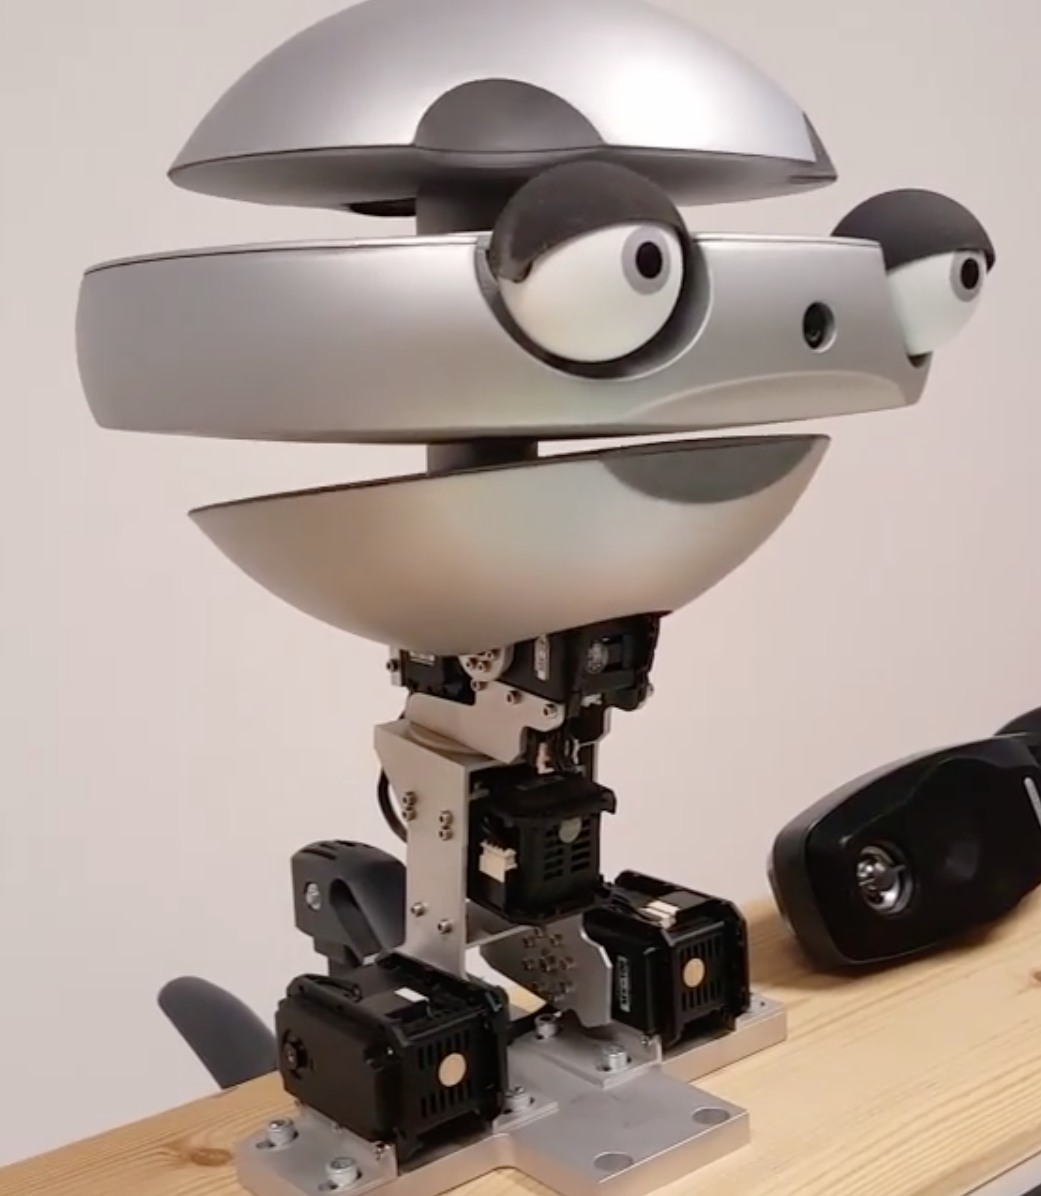
\includegraphics[width=0.4\textwidth]{images/emys.png}}
		\caption{EMYS robot.}
		\label{fig:robots:EMYS}
	\end{minipage}
%	\hfill
	\begin{minipage}[b]{.4\textwidth}
		\centering
		\frame{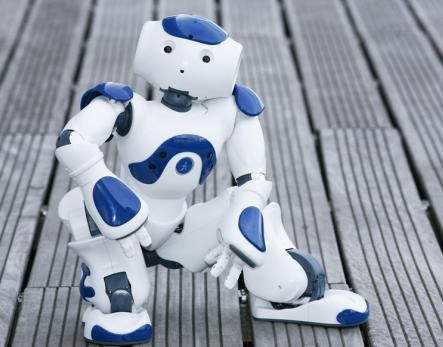
\includegraphics[width=0.55\textwidth]{images/NAO_Robot.JPG}}
		\caption{NAO robot.}
		\label{fig:robots:NAO}
	\end{minipage}
\end{figure}